\section{Introduction}

\setLayout{mainpoint}

\begin{frame}[noframenumbering, plain]{}
    \frametitle{Introduction}
\end{frame}

\setLayout{vertical}

%---------------------------------------------------------
\begin{frame}{Cell Cultures}
    \begin{itemize}
        \item Vital to industrial and academics applications.
        \item Key part in drug discovery and development:
        \begin{itemize}
            \item Pre-Clinical.
            \item Clinical.
        \end{itemize}
    \end{itemize}
\end{frame}

%---------------------------------------------------------
\begin{frame}{Drug Discovery}
    \begin{figure}[!htb]
    \centering
    \subfloat[\textit{in silico}]{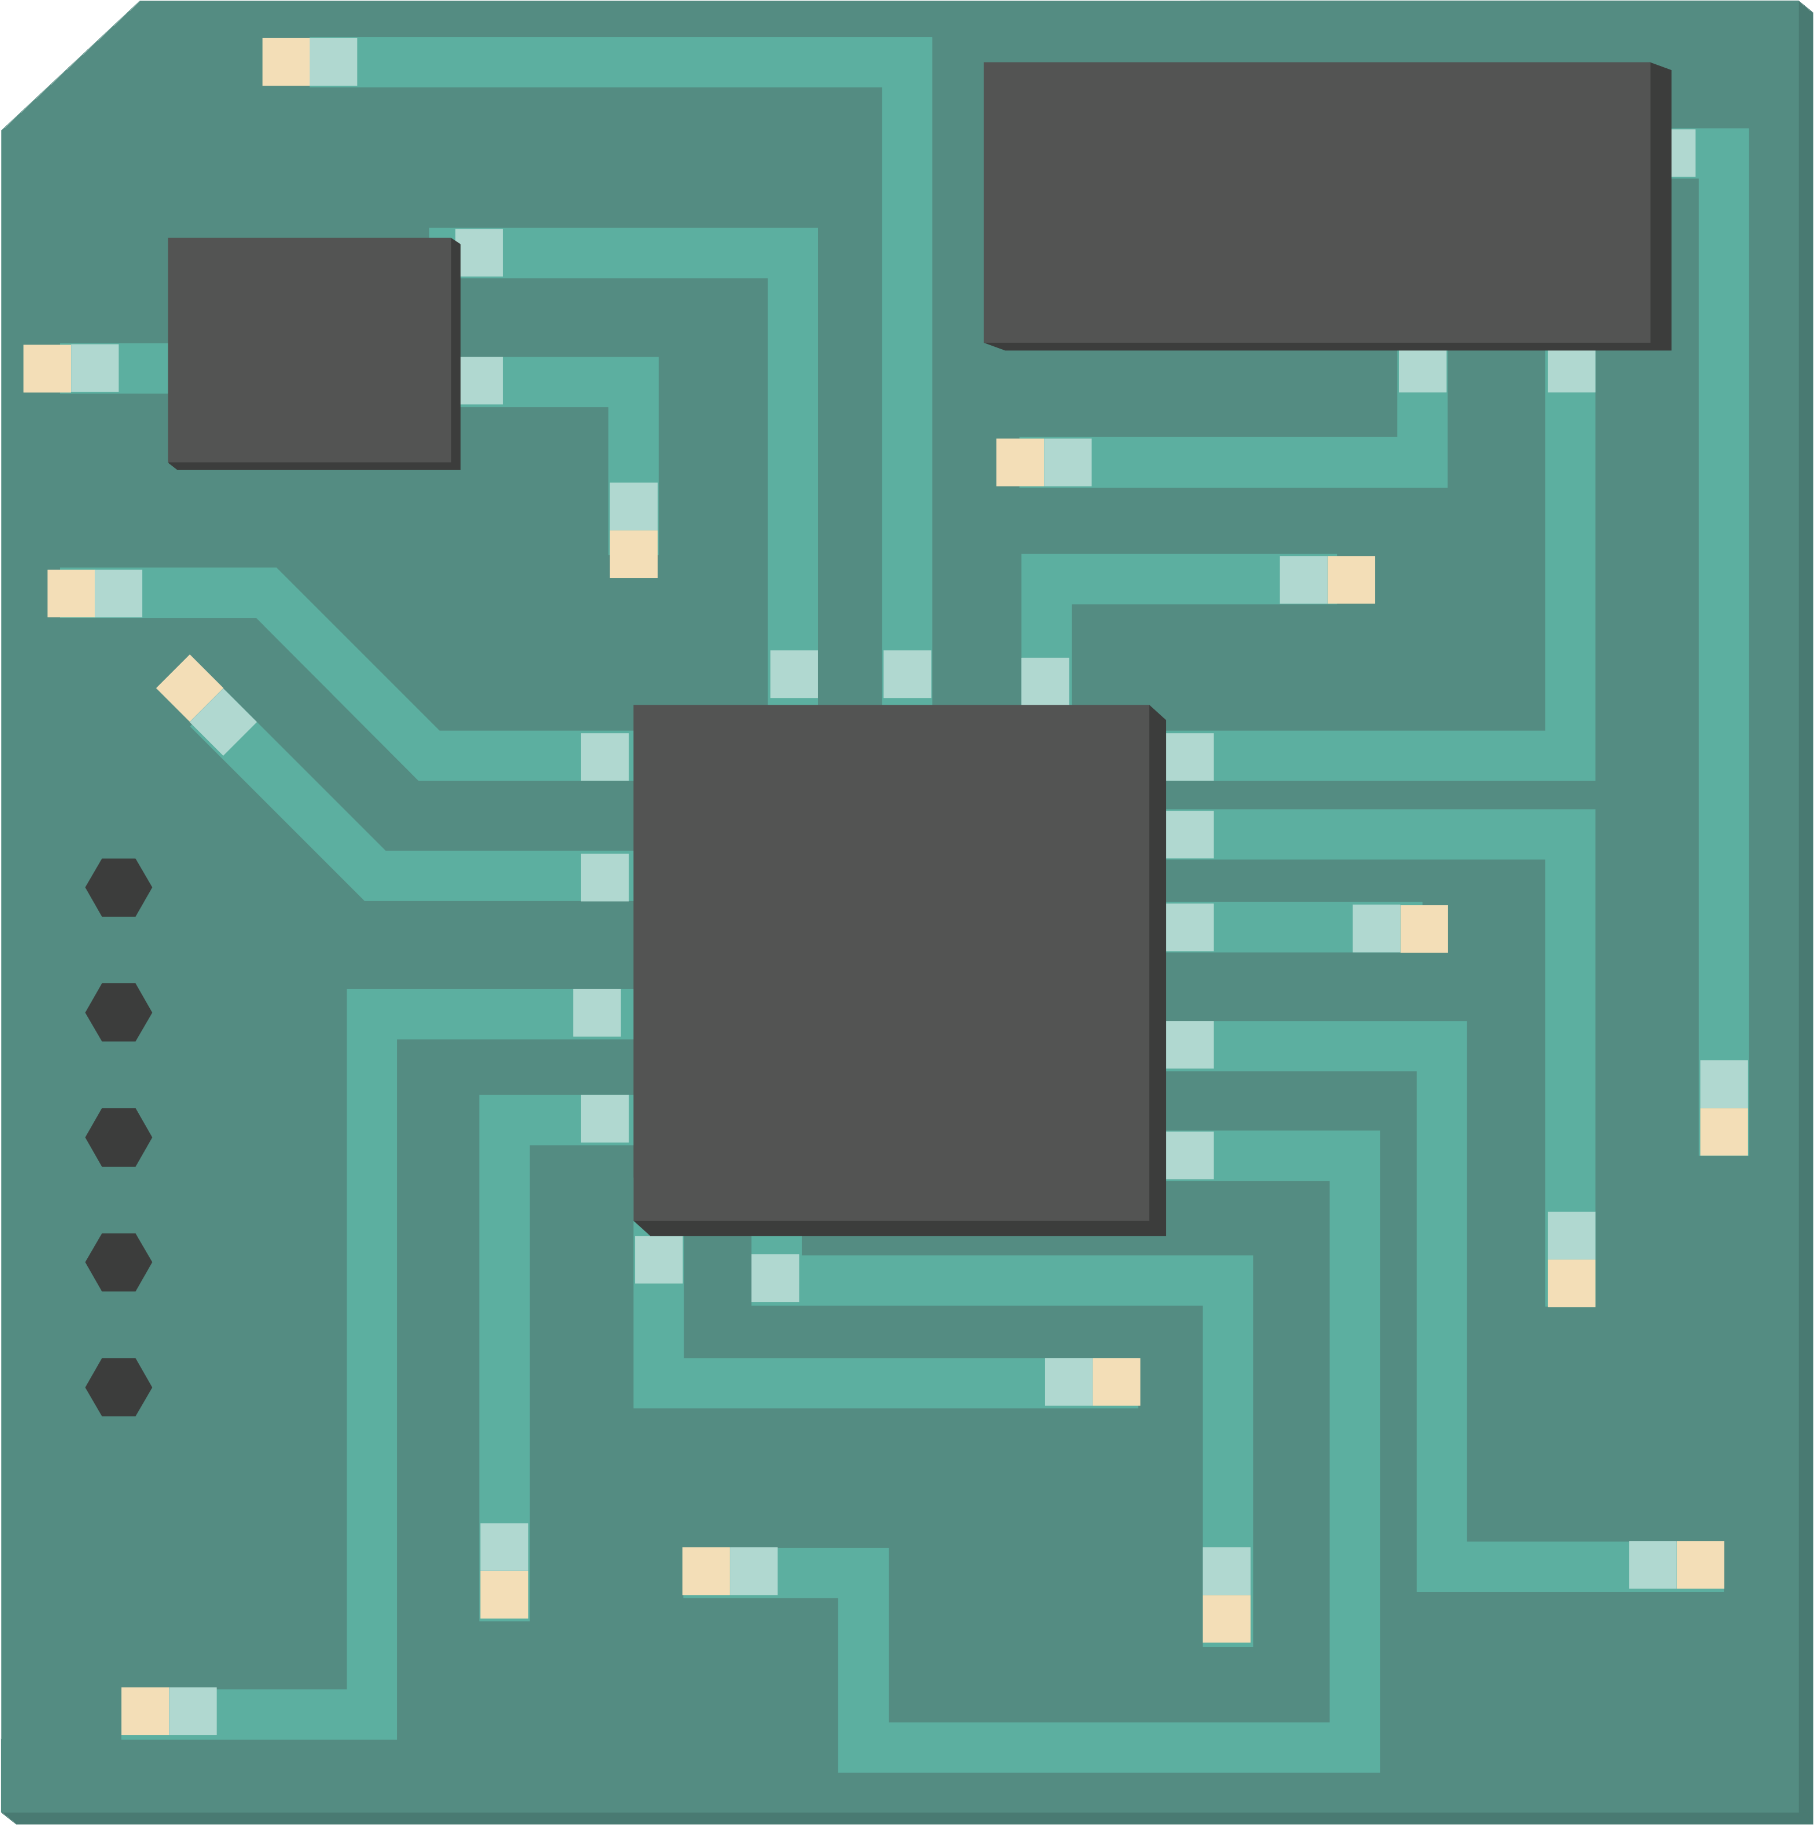
\includegraphics[width=2cm]{figures/introduction/in_silico} \label{fig:in_silico}} \hspace*{0.3cm}
    \subfloat[\textit{in vitro}]{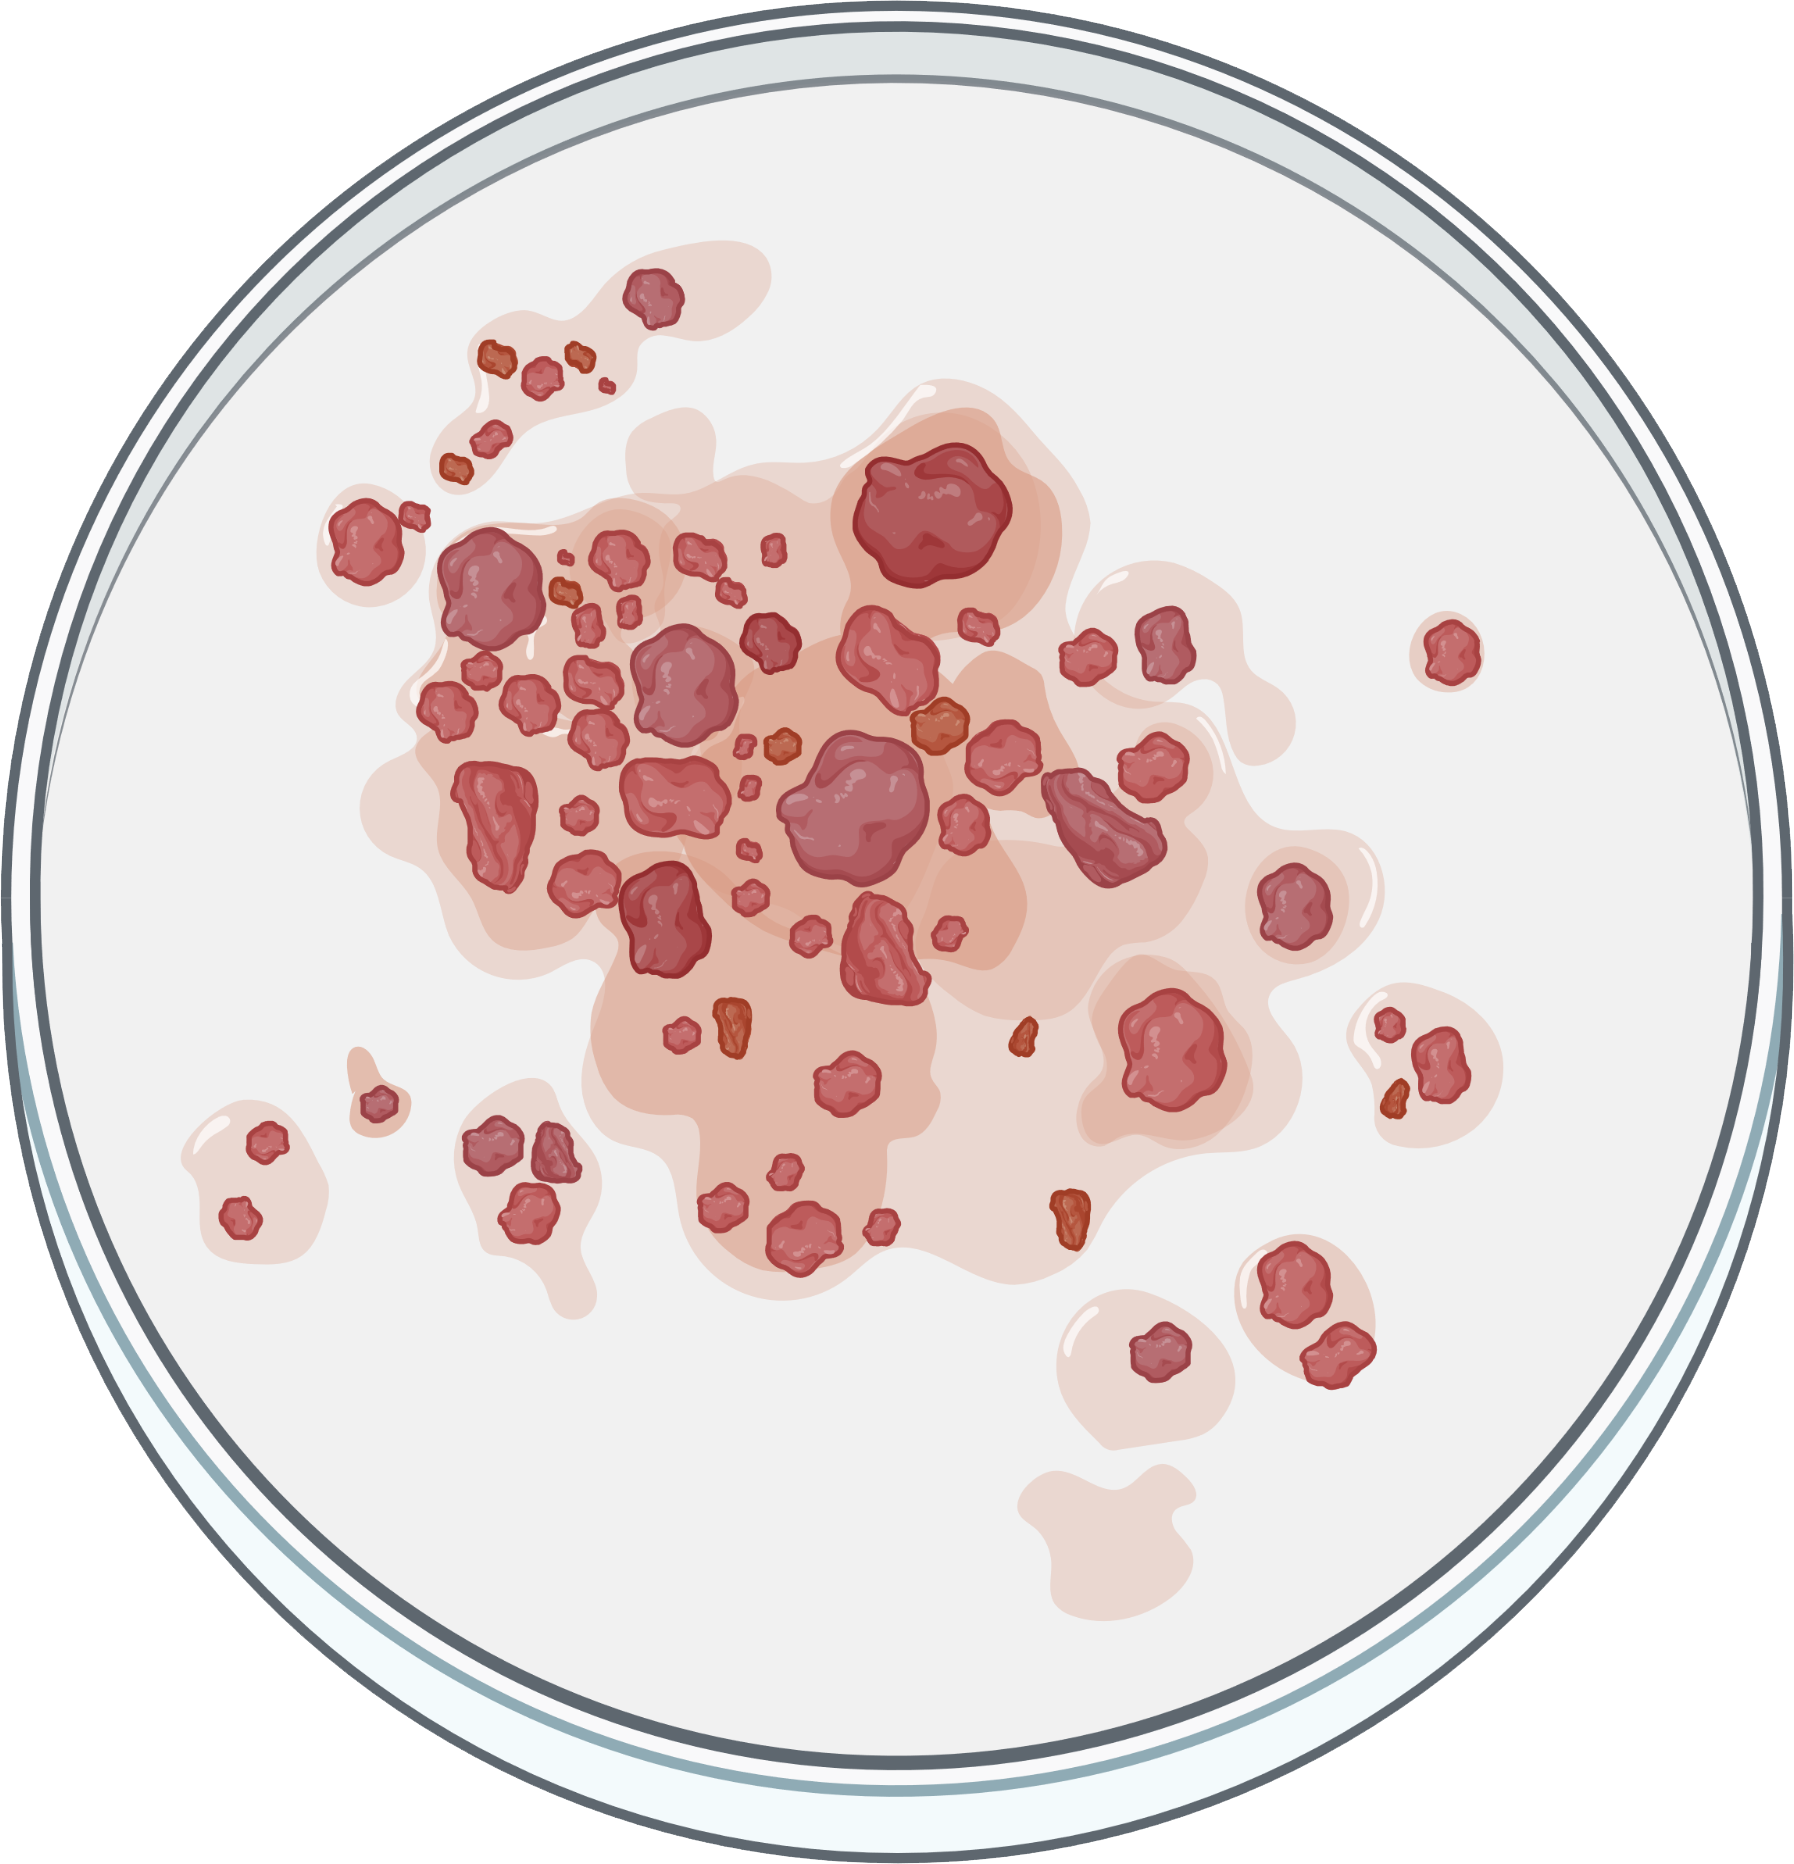
\includegraphics[width=2cm]{figures/introduction/in_vitro} \label{fig:in_vitro}} \hspace*{0.3cm}
    \subfloat[\textit{in vivo}]{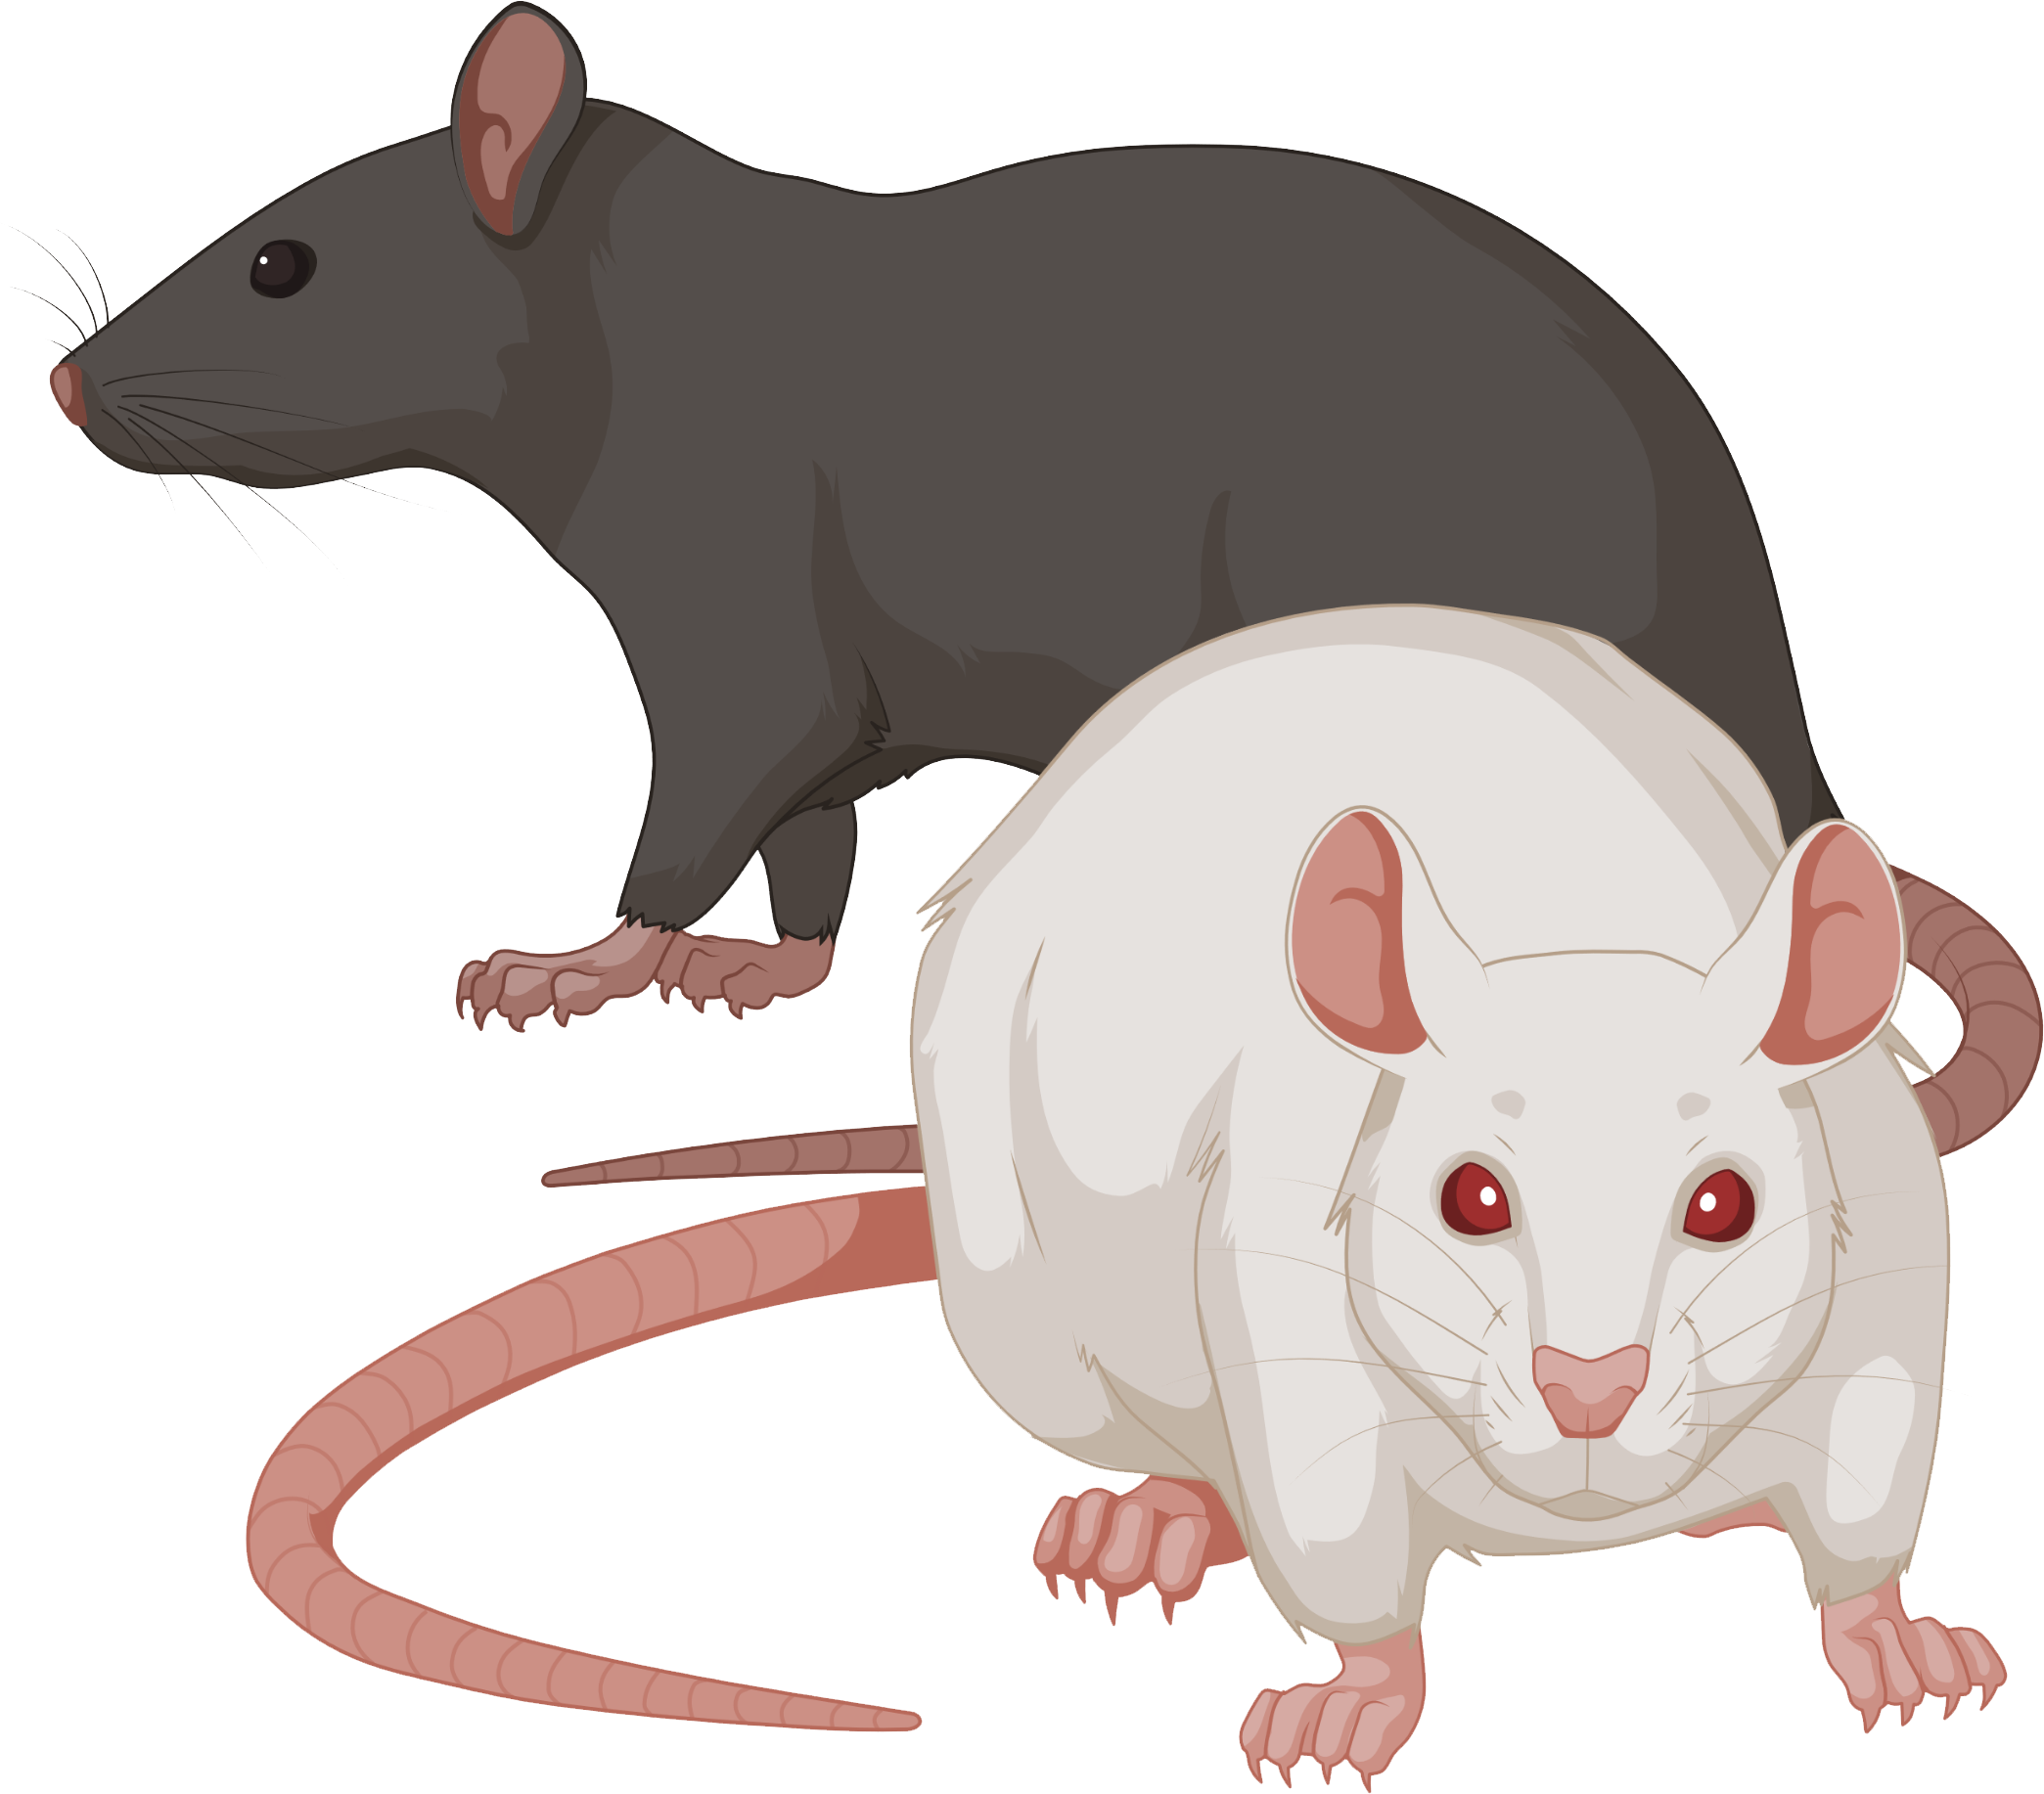
\includegraphics[width=2cm]{figures/introduction/in_vivo} \label{fig:in_vivo}}\\
    \subfloat[Clinical Trials]{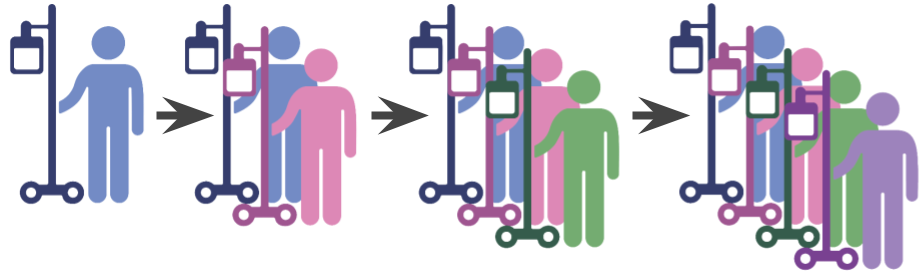
\includegraphics[width=9cm]{figures/introduction/clinical} \label{fig:clinical_trials}}
    \label{fig:introduction_drug_trials}
    \end{figure}
\end{frame}

%---------------------------------------------------------
\begin{frame}{2D \textit{vs} 3D}
    \begin{figure}[!htb]
    \centering
    \subfloat[\textit{2D culture}]{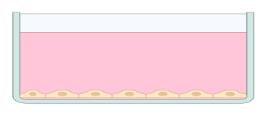
\includegraphics[width=6cm]{figures/introduction/2D_culture} \label{fig:2d_culture}} \hspace*{0.3cm}
    \subfloat[\textit{3D culture}]{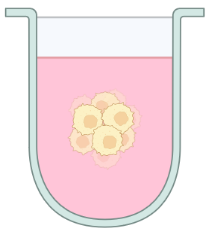
\includegraphics[width=4cm]{figures/introduction/3D_culture} \label{fig:3d_culture}} \hspace*{0.3cm}
    \label{fig:2d_vs_3d}
    \end{figure}
\end{frame}

%---------------------------------------------------------
\begin{frame}{Spheroid Regions}
    \begin{figure}
        \centering
        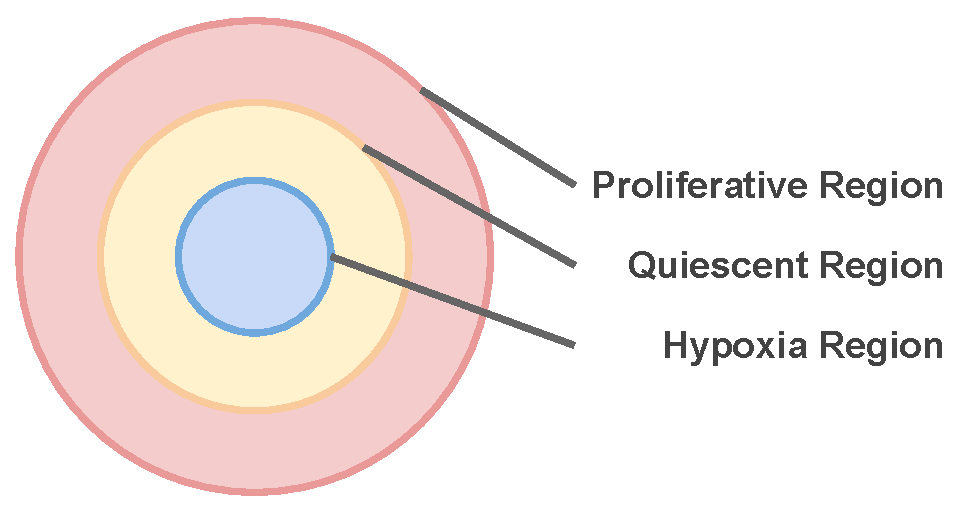
\includegraphics[width=8cm]{figures/introduction/spheroid_regions}
        \label{fig:spheroid_regions}
    \end{figure}
\end{frame}

%---------------------------------------------------------
\begin{frame}{Research Questions}
        \begin{enumerate}
            \item Shape-aware \alert{loss function affects} segmentation?
            \item Is the U-net encoder a \alert{better generator backbone} for spheroid segmentation?
            \item Can we evaluate spheroids with \alert{destroyed proliferative zones}?
            \item Is \alert{scale} important in spheroid segmentation?
            \item Can a single GAN \alert{differentiate all three spheroid zones}?
        \end{enumerate}
\end{frame}

%---------------------------------------------------------
\setLayout{horizontal}

\begin{frame}{Objectives}
    \begin{columns}
        \column{0.5\textwidth}
            \begin{block}{Global Objectives}
                \begin{enumerate}
                    \item Create the spheroid image dataset (SDSS).
                    \item A self-supervised semantic segmentation method.
                \end{enumerate}
            \end{block}
        \column{0.5\textwidth}
            \begin{block}{Specific Objectives}
                \begin{enumerate}
                    \item Literature review.
                    \item Setup dataset.
                    \item Select metric.
                    \item Develop method.
                    \item Evaluate Loss functions.
                    \item Select GAN backbones.
                    \item Process results.
                \end{enumerate}
            \end{alertblock}
    \end{columns}
\end{frame}

%---------------------------------------------------------
\setLayout{vertical}

\begin{frame}{Expected Challenges}
    \begin{itemize}
        \item Access to data.
        \item Lack of protocols.
        \item Heterogeneous evaluation metrics.
        \item GANs convergence.
        \item Annotate images.
        \item Train with few samples.
    \end{itemize}
\end{frame}

%---------------------------------------------------------
\begin{frame}{Expected Contributions}
    \begin{itemize}
        \item New public dataset.
        \item New self-supervised segmentation method.
        \item Segmentation as an analysis tool.
        \item Qualitative study.
        \item Competitive results.
    \end{itemize}
\end{frame}
